
\documentclass[preprint,12pt]{elsarticle}
\journal{Computers and Mathematics with Applications}
\newtheorem{theorem}{Theorem}[section]
\newtheorem{lemma}[theorem]{Lemma}
\newtheorem{proposition}[theorem]{Proposition}
\newtheorem{corollary}[theorem]{Corollary}
\newtheorem{claim}[theorem]{Claim}
\newtheorem{definition}[theorem]{Definition}

\usepackage{multicol,amsmath,amssymb,latexsym,amsfonts}
\usepackage{paralist}

%
% MCs commands
\newcommand{\x}{{\bf x}}
\newcommand{\n}{{\bf n}}
\newcommand{\y}{{\bf y}}
\newcommand{\w}{{\bf w}}
\newcommand{\E}{{\bf E}}
\newcommand{\s}{{\bf s}}
\newcommand{\z}{{\bf z}}
\newcommand{\RR}{{\mathbb{R}}}
\newcommand{\ZZ}{{\mathbb{Z}}}
\newcommand{\xx}{{\mathbf{x}}}
\newcommand{\yy}{{\mathbf{y}}}
\newcommand{\zz}{{\mathbf{z}}}
\newcommand{\del}{{\mathbb{\triangledown}}}

%
% Bryan's commands
\newcommand{\pderiv}[2]{\frac{\partial #1}{\partial #2}}
\newcommand{\pderivtwo}[2]{\frac{\partial^{2} #1}{\partial #2 ^{2}}}
\newcommand{\bd}{{\partial}}
\newcommand{\eqr}[1]{~(\ref{#1})}
\newcommand{\figr}[1]{figure~\ref{#1}}
\newcommand{\figrs}[1]{figures~\ref{#1}}
\newcommand{\Figr}[1]{Figure~\ref{#1}}
\newcommand{\Figrs}[1]{Figures~\ref{#1}}
\newcommand{\tabr}[1]{table~\ref{#1}}
\newcommand{\Tabr}[1]{Table~\ref{#1}}
\newcommand{\sref}[1]{\S~\hspace{-3pt}\ref{#1}}
% Use the option doublespacing or reviewcopy to obtain double line spacing

 %\documentclass[doublespacing]{elsart}

% if you use PostScript figures in your article
% use the graphics package for simple commands
 \usepackage{graphicx}
 \usepackage{subfigure}
% \usepackage{lineno}
% or use the graphicx package for more complicated commands
% \usepackage{graphicx}
% or use the epsfig package if you prefer to use the old commands
% \usepackage{epsfig}

% The amssymb package provides various useful mathematical symbols
\begin{document}
% The lineno packages adds line numbers. Start line numbering with
% \begin{linenumbers}, end it with \end{linenumbers}. Or switch it on
% for the whole article with \linenumbers.

% \linenumbers

% Title, authors and addresses

% use the thanksref command within \title, \author or \address for footnotes;
% use the corauthref command within \author for corresponding author footnotes;

% use the ead command for the email address,
% and the form \ead[url] for the home page:
\begin{frontmatter}

\title{Fast integral equation methods for Rothe's method applied to the isotropic heat equation}
 \author{Mary Catherine A. Kropinski\corref{nserc}\fnref{mcak}}
 \author{Bryan D. Quaife\fnref{mcak}}
 \address[mcak]{Department of Mathematics, Simon Fraser University,
 Burnaby, British Columbia, Canada V5A 1S6}
% \ead{mkropins @ cs.sfu.ca}
% \ead[url]{home page}
 \cortext[nserc]{Supported in part by Natural Sciences and Engineering Research Council of Canada Grant RGPIN 203326}

\begin{abstract}
We present an efficient integral equation approach to solve the forced heat equation, $u_t (\x) - \Delta u(\x) = F(\x, u, t)$, in a two-dimensional, multiply connected domain, with Dirichlet boundary conditions. Instead of using an integral equation formulation based on the heat kernel, we discretize in time, first. This approach, known as Rothe's method, leads to a non-homogeneous modified Helmholtz equation that is solved at each time step. We formulate the solution to this equation as a volume potential plus a double layer potential, and both of these potentials are calculated with available tools accelerated by the fast multipole method. For a total of $N$ points in the discretization of the boundary and the domain, the total computational cost per time step is $O(N)$. We demonstrate our approach on the heat equation and the Allen-Cahn equation. 
\end{abstract}

\begin{keyword}
% keywords here, in the form: keyword \sep keyword
fast multipole method \sep Gaussian quadrature \sep modified Helmholtz
equation \sep integral equations \sep the heat equation \sep Rothe's method \sep Allen-Cahn equation.
% PACS codes here, in the form: \PACS code \sep code
%\PACS
\end{keyword}
\end{frontmatter}

\section{Introduction}
Integral equation methods offer an attractive alternative to conventional finite difference and finite elements for solving partial differential equations that arise in science and engineering. 
They offer several advantages: complex physical boundaries are easy to incorporate, the ill-conditioning associated with directly discretizing the governing equation is avoided, high-order accuracy is easier to attain, and far-field boundary conditions are handled naturally.
Nevertheless, integral equation methods have been slow to be adopted for larger-scale problems, and the  reason for this is clear: on an $N\times N$ mesh, integral equation formulations lead to systems with dense $N^2 \times N^2$ matrices.
This situation is further exacerbated if the problem is time dependent. 

In recent years, fast algorithms have been developed for integral equations for a variety of elliptic boundary value problems that are closely related to the methods we will discuss here. An early example is the work by Greenbaum et al. in \cite{mult:conn} for Laplace's equation in multiply connected domains.
Subsequently, similar tools were developed for Poisson's equation \cite{greengard:ethridge}, the Stokes equations \cite{stokes:flow}, and the modified Helmholtz equation \cite{modified:helmholtz,KROP_QUAIFE_1}. 
All of these approaches are characterized by the following: well-conditioned integral-equations, if needed, are formulated, integrals are discretized using high-order quadrature, and the resulting linear systems are solved or evaluated using a fast multipole-accelerated iterative solver. As a result, these tools are highly accurate and have optimal efficiency: for $N$ points in the discretization of the boundary or domain, the solution procedure requires only $O(N)$ operations. 

The development of corresponding algorithms for time-dependent problems, however, is considerably more complex. There is a substantial literature on integral equation methods for the heat equation. However, standard discretizations of these integral equations leads to very expensive methods, as the solution depends on the full space-time history.  For $N$ points in the discretization of the domain and $M$ time steps, the computational cost requires $O(N^2M + N^2 M^2)$ operations \cite{heat_solver_1}.  There is recent work by Li and Greengard in \cite{heat_solver_1,heat_solver_2} on developing fast solvers for the heat equation. Their methods use an integral equation formulation based on the heat kernel and rely on a non-uniform FFT.  While robust, this approach is highly complicated. Methods that rely on a fast Gauss transform are discussed in \cite{tausch,SKVandGB,SKVandGB2}.
(For a more thorough overview of fast-multipole accelerated integral equation methods, see \cite{nishimura}.) 

We present an alternative approach which relies on available fast algorithms for elliptic problems. 
A semi-implicit temporal discretization of a convection-diffusion-type equation yields the modified Helmholtz, or linearized Poisson-Boltzmann, equation
\begin{equation}
  u(\x) - \alpha^2 \Delta u(\x) = B(\x,u,t),
  \label{eq:mod_lap_hom}
\end{equation}
where $\alpha^2 = O(\Delta t)$. 
Thus the parabolic heat equation is solved as a sequence of elliptic boundary value problems, and this approach is known as {\it Rothe's method}.
In general, an integral equation formulation for solutions to\eqr{eq:mod_lap_hom} will require both a layer and volume potential. 
In \cite{chapko_kress}, Chapko and Kress present a boundary-only integral equation formulation for Rothe's method applied to the heat equation. Chapko applies a similar approach to the unsteady Stokes equations in \cite{chapko}.
However, their boundary-integral formulation applies only to homogeneous equations with homogeneous initial conditions. We aim to solve problems in a more general setting for which including a volume potential is unavoidable. 

We base our solver on coupling two fast computational tools for the operator $(1-\alpha^2 \Delta)$. 
In \cite{modified:helmholtz}, Cheng et al. present a fast direct solver for\eqr{eq:mod_lap_hom} in two dimensions on the unit square.  
The solution is expressed as a volume potential, and the direct solver is accelerated using a new version of the fast multipole method \cite{screened_coulomb, new_FMM}. 
The solver is fully adaptive and the computational costs are comparable to those of FFT-based methods.
In \cite{KROP_QUAIFE_1}, we present fast, well-conditioned integral equation methods for solving the homogeneous equation in unbounded and bounded multiply-connect domains, with either Dirichlet or Neumann boundary conditions. 
In this paper, we present a preliminary study on coupling the methods discussed in \cite{modified:helmholtz} to those discussed in \cite{KROP_QUAIFE_1} in order to solve nonlinear diffusion-type problems in complicated domains. In order to simplify our focus, we consider problems in bounded multiply-connected domains with constant Dirichlet boundary conditions. 
The purpose of this paper is twofold: To demonstrate that our approach has the potential to efficiently and accurately solve nonlinear diffusion-type problems in complicated two-dimensional domains, and to identify the key issues that will require more investigation in order to develop a more general solver. 
Once fully realized, our approach will have the following features:
\begin{itemize}
\item High-order temporal schemes will be easily implemented.
\item The difficulty and expense associated with convolutions involving the heat kernel will be avoided. 
\item Spatial adaptivity for resolving features on the boundary and in the domain will be easily incorporated.
\item The expense associated with generating an unstructured mesh for complicated geometry will be avoided.  
\item The solution will be based entirely on an integral formulation, resulting in a well-conditioned method.
\item High-order quadrature will be used, resulting in a scheme that has high spatial accuracy. 
\item The FMM-accelerated solution procedure will have optimal or near-optimal efficiency.
\end{itemize}

There are integral-equation based methods that are also well suited for the problem at hand. Our approach closely resembles the methods presented by Biros et al. in \cite{BIROS} for the Stokes equations and which were extended to the Navier-Stokes equations in \cite{GB_LY_DZ}. 
Their method is called an {\it embedded boundary integral} method (EBI) which is an extension of the techniques developed by Mayo in \cite{mayo} for efficiently evaluating the volume potentials for the Laplace and biharmonic equations. 
Instead of integrating in order to evaluate the volume potential, these approaches are based on a finite difference or finite element method with locally corrected stencils to account for jumps in the solution values across the interface or physical boundaries. 
In \cite{GB_LY_DZ,BIROS,mayo} a second-order method is used, although this approach has been extended to 4th order and recently to three dimensions \cite{MAYO_2,mayo_greenbaum}.
The EBI method has the advantage of being easier to implement - an advantage which becomes even more critical when moving to three dimensions. However, in the case of the Navier-Stokes equations, there is some indication that the differencing of the convection term leads to more severe time-step constraints as the Reynold's number increases (cf.  \cite{GB_LY_DZ}). This is less problematic when using a purely integral formulation (cf. \cite{int:equation:nse}), although this point warrants closer examination.
Another method would be to generate an unstructured mesh in order to calculate the volume potential.  However, we wish to avoid the difficulties associated with mesh generation and work with an approach that is naturally adaptive and will extend readily to three dimensions.  

The paper is organized as follows: In Section 2, we discuss the temporal discretization of the heat equation and how this gives rise to the modified Helmholtz equation. 
We outline the corresponding potential theory for the modified Helmholtz equation: the solution is decoupled into the sum of a volume potential and double layer potential with an unknown density, and an integral equation for the unknown layer density is formulated. In Section 3,
numerical methods for the evaluation of the volume potential and the integral equation are 
discussed. 
Numerical examples are presented in Section 4.

\begin{figure}[t]
     \centering
$\begin{array}{c}
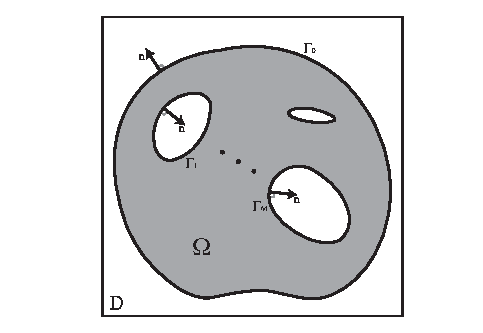
\includegraphics[height=2in]{figure1.eps}
\end{array}$
  \caption{\em A  bounded $(M+1)$-multiply-connected domain $\Omega$ (in gray) is embedded in the unit square $D$.  The outer boundary is denoted by $\Gamma_0$, the interior component 
    curves by $\Gamma_1,\ldots,\Gamma_M$,  $\Gamma$ is the union of all such curves, $\Omega_k$, $k=1,\ldots,M$ is the region in $D$ bounded by $\Gamma_k$, and $\Omega_0 = D\backslash \Omega_1 \cup \cdots \cup \Omega_M$.The unit normal $\n$ points out of $\Omega$ (and into $D\backslash \Omega$) on each component curve.}
  \label{fig1}
\end{figure}
%%%%%%%%%%%%%
\section{Potential theory and the integral equation formulation}
To fix notation, let us consider a $(M+1)$-ply connected bounded domain $\Omega$ with boundary $\Gamma$ which is comprised of individual smooth component curves $\Gamma_k$ (see \figr{fig1}). Consider the isotropic inhomogeneous heat equation in $\mathbb{R}^2$:
\begin{equation}
  u_t(\x,t) -\Delta u(\x,t) = F(\x,u,t),  \qquad  \x \in \Omega, \; t>0,  \label{pde} 
\end{equation}
with Dirichlet boundary conditions:
\[
  u(\x,t) =  f(\x,t), \qquad  \x \in \Gamma, \; t>0, 
\]
and initial condition
\[
  u(\x,0) = u_0(\x), \qquad  {\x} \in \Omega.  
\]
In order to prevent a severe time-step restriction, linearly implicit or IMEX schemes \cite{Ruuth} are generally used for marching in time. 
In such schemes, the diffusive term is treated implicitly, while the remainder is treated explicitly.
Regardless of the details of the particular choice of IMEX scheme, the temporal discretization of\eqr{pde} yields the modified Helmholtz equation:
\begin{equation}
\begin{array}{rcll}
  u^{N+1} - \alpha^2 \Delta u^{N+1} & = &  B(\x, t^N, t^{N-1}, \cdots,  u^N,u^{N-1},\cdots), & {\x} \in \Omega,  \smallskip \\
  u^{N+1} & =  & f(\x,t), &  \x \in \Gamma, \smallskip \\
  u^0 & =  & u_0(\x), &  \mbox{at } t = 0,
 \end{array}
\label{mod_helm_forced} 
\end{equation}
where $t=(N+1) \Delta t$ is the current time.
The simplest such scheme is the first-order backward Euler method, which is of the form\eqr{mod_helm_forced} with   
\[
   \alpha^2 =  \Delta t, \qquad B = u^N + \Delta t F^N. 
\]
A second-order method is the extrapolated Gear method (herein referred to as SBDF), for which
\[
\alpha^2 =  \frac{2}{3} \Delta t, \qquad B = \frac{4}{3} u^N -\frac{1}{3} u^{N-1}+
                 \frac{4}{3}  \Delta t F^N  - \frac{2}{3} \Delta t F^{N-1}. \label{exg}
\]
At each time step, we represent the solution to\eqr{mod_helm_forced} as
\[
U(\x) = U^p(\x) + U^h(\x).  
\]
Here, $U^p$ satisfies
\begin{equation}
   U^p - \alpha^2 \Delta U^p = B, \qquad    \x \in \Omega, 
   \label{particular}
\end{equation}
and $U^h$ satisfies
\begin{equation}
   \begin{array}{rcll}
   U^h  - \alpha^2 \Delta U^h & = & 0, &   \qquad \x \in \Omega, \smallskip \\
   U^h & =  & g(\x) , &   \qquad \x \in \Gamma,  
   \end{array}
 \label{mod_helm_hom}
\end{equation}
where $g(\x) =  f(\x) - U^p(\x)$.

The fundamental solution to the modified Helmholtz equation is 
\[
  G(\x) = \frac{1}{2\pi\alpha^2} K_0 \left( \frac{|\x|}{\alpha} \right), 
\]
where $K_0$ is the zeroth-order modified Bessel function of the second
kind. In other contexts, $G(\x)$ is also referred to as the Yukawa or screened Coulomb potential. 
We represent the solution to\eqr{particular} as a volume potential: 
\begin{equation}
   U^p(\x) = \frac{1}{2\pi\alpha^2}\int_\Omega B(\y) K_0 \left( \frac{|\y - \x|}{\alpha} \right) \, dA_{\y}. \label{vol_potential}
\end{equation}
We seek the solution to\eqr{mod_helm_hom} in the form of a double layer potential
\begin{equation}
  U^h(\x)=\frac{1}{2\pi\alpha^2}\int_{\Gamma}\pderiv{}{n_{\y}}K_{0}
  \left(\frac{|\y-\x|}{\alpha} \right) \sigma(\y) ds(\y), \qquad \x\in\Omega, \label{eqn:dlp}
\end{equation}
where  $\sigma(\y)$ is the value of an unknown
density at the boundary point $\y$, and $\partial / \partial n_\y$
represents the outward normal derivative at the point $\y$.
The unknown density $\sigma$ is found by solving an integral equation derived to ensure the boundary condition in\eqr{mod_helm_hom} is satisfied. 

In \cite{KROP_QUAIFE_1}, we derive integral equation formulations to solve\eqr{mod_helm_hom} in bounded and unbounded multiply-connected domains for both Neumann and Dirichlet boundary data. 
Here, we summarize the results for the bounded case with Dirichlet boundary conditions.  
Observing that $K_0 (z) \sim -\log(z)$ as $z \rightarrow 0$ \cite{ABRAM}, 
we can determine the jump relations of the double layer potential as these are well known for the logarithmic kernel. 
Thus for any point $\x$ on the smooth boundary $\Gamma$,
\begin{eqnarray*}
  \lim_{\tiny{\begin{array}{l}
        \x'  \rightarrow  \x  \\
        \x'  \in  \Omega 
      \end{array} }}
  U^h(\x')& = &  - \frac{1}{2\alpha^2}\sigma(\x)+
  \frac{1}{2\pi\alpha^2}\int_{\Gamma}\pderiv{}{n_{\y}}
  K_{0}\left(\frac{|\y-\x|}{\alpha}\right)\sigma(\y)ds(\y).
\end{eqnarray*}
Substituting the above into the boundary condition in\eqr{mod_helm_hom} results in the integral equation 
\begin{equation}
  \label{dirichlet:inteqn}
 -\frac{1}{2\alpha^2}\sigma(\x)+\frac{1}{2\pi\alpha^2}
  \int_{\Gamma}\pderiv{}{n_{\y}}K_{0}\left(\frac{|\y - \x|}{\alpha}\right)
  \sigma(\y) \, ds(\y) = g(\x) .
\end{equation}
As we discuss in \cite{KROP_QUAIFE_1}, the kernel in the above is continuous along
$\Gamma$, 
\[
  \lim_{\tiny{\begin{array}{r}\y \rightarrow \x \smallskip \\
        \x, \y \in \Gamma
      \end{array} }}
  \pderiv{}{n_{\y}}K_{0}\left(\frac{|\y-\x|}{\alpha}\right) = 
  -\frac{1}{2}\kappa(\x),
\]
where $\kappa(\x)$ denotes the curvature of $\Gamma$ at the point
$\x$.
Summarizing, the kernel in the integral equation is bounded and continuous, and the integral operator is therefore compact. In addition, there are no nontrivial
homogeneous solutions. By the Fredholm alternative,\eqr{dirichlet:inteqn} has a unique solution for any integrable data
$g(\x)$.
%%%%%%%%%%%%%
\section{Numerical methods}
We now discuss our numerical procedure.
In Section 3.1, we first outline the methods involved in evaluating the volume potential\eqr{vol_potential}. 
Next, in Section 3.2, we discuss the coupling of the volume potential to the double layer potential through the boundary conditions and solving the corresponding integral equation\eqr{dirichlet:inteqn}. 
While the FMM plays an integral role in our numerical methods, its implementation is standard and has been discussed at length in other works. 
For details on the FMM, we refer the reader to the work in \cite{GR,CGR} for the original FMM, \cite{new_FMM} for the new FMM algorithm based on exponential expansions to represent the far-field interactions, and \cite{modified:helmholtz} for the FMM applied to the modified Helmholtz equation in two dimensions.
In Section 3.3, the entire solution procedure taken per time step is summarized.

\subsection{The volume potential}
In \cite{modified:helmholtz}, methods for the rapid evaluation of the volume potential for the modified Helmholtz equation on the unit square were discussed.
These methods use adaptive mesh refinement, and the evaluation is accelerated using the new version of the FMM. 
In order to employ these methods, we must first extend the right-hand side of\eqr{pde}, which is defined only in $\Omega$ to be defined throughout $D$. 
One naive way to define an extension $\tilde{B}(\x,t,u)$ of $B(\x,t,u)$ is the following: 
\[
   \tilde{B}(\x,t,u) = \left\{ \begin{array}{rl}
                                       B(\x,t,u), & \qquad \x \in \Omega \\
                                       0, & \qquad \x \in D \backslash  \Omega.
                                    \end{array} \right.
\]
However, the discontinuity across $\Gamma$ would likely cause excessive grid refinement in the vicinity of the boundary, and consequently slow down the evaluation (cf. example 4.4 in \cite{greengard:ethridge}; up to $O(10^5)$ grid points are needed to solve $\Delta u=1$ inside a disk and $\Delta u = 0$ outside). 
For multiple-component boundaries, this would simply become too expensive. 

For our purposes here, we consider problems in which the boundary conditions on each $\Gamma_k$ are constant, and in addition, $F$ does not depend explicitly on $t$ or $\x$, i.e. $F = F(u)$. Consequently, $B$ also does not depend explicitly on $t$ or $\x$ and a continuous ${\tilde B}$ can easily be constructed. 
We save the important consideration of an extension of $B$ in the case of general boundary conditions for future work.
Define $\Omega_k$, $k=1,\ldots,M$ to be the region in $D$ bounded by $\Gamma_k$, and $\Omega_0 = D\backslash \Omega_1 \cup \cdots \cup \Omega_M$ (see \figr{fig1}). 
Assume the Dirichlet boundary conditions are given by $u=C_k$ on $\Gamma_k$ for $k=0,\ldots,M$. 
Then, we define $\tilde{B}$ by:
\[
   \tilde{B}(u) = \left\{ \begin{array}{rl}
                                       B(u), & \qquad \x \in \Omega, \\
                                       B(C_k), & \qquad \x \in \Omega_k, \\
                                       B(C_0), & \qquad \x \in \Omega_0.
                                    \end{array} \right.
\]
We now outline the methods presented in \cite{modified:helmholtz} to evaluate
\begin{equation}
   \tilde{U}^p(\x) = \int_D\tilde{B}(\x,t) G(\y - \x) \, dA_{\y}.   \label{volume_potential}
\end{equation}

The FMM uses an adaptive quadtree structure in order to superimpose a hierarchy of refinement on the computational domain. 
The unit square $D$ is considered to be grid level 0. Grid level $l+1$ is obtained recursively by subdividing each square (or node) $s$ at level $l$ into four equal parts; these are called the ``children'' of $s$. 
Adaptivity is achieved by allowing different levels of refinement throughout the tree.
The square $s$ is refined if the error of a third-order polynomial interpolating $\tilde{B}$ is larger than some preset tolerance, $\tau$ (the interpolation is checked at 64 points within $s$).  
We denote the childless nodes in the quadtree as $D_i$, $i=1, \ldots, P$, where $P$ is the total number of such nodes. 
We assume we are given $\tilde{B}$ on a cell-centered $4\times 4$ grid for each $D_i$. 
Thus, $N_D = 16 \times P$ is the total number of grid points in $D$. 
To obtain fourth-order accuracy, these 16 points are used to construct a third-order polynomial to $\tilde{B}$ of the form
\[
  \tilde{B}(\x) \approx \sum_{j=1}^{10} c^i_j \, p_j (\x-\x^i), \qquad \x \in D_i, 
\] 
where $\x^i$ is the centre of $D_i$ and $\{ p_{j} \}$ are the standard basis functions for polynomials up to
order three
(see \cite{modified:helmholtz,greengard:ethridge} for details on the approximating polynomial).
Therefore, the evaluation of\eqr{volume_potential} is approximated by 
\[
  \tilde{U}^p (\x) \approx \sum_{i=1}^P 
    \int_{D_i} G(\y - \x ) \, \sum_{j=1}^{10} c^i_j \, p_j (\y-\x^i) \, dA_{\y} .
 \]
Direct evaluation of this potential at all $N_D$ grid points would require $O(N^2_D)$ work. 
This expense is reduced to $O(N_D)$ work, by using the FMM.

\subsection{The integral equation}
We now discuss the numerical methods to solve\eqr{dirichlet:inteqn}.
We assume each component curve $\Gamma_k$, $k=0,\ldots, M$ is
parametrized by $\y^k(\alpha)$, where $\alpha \in [0, 2\pi)$. Similarly, $\sigma^k(\alpha)$ refers to the restriction of the density $\sigma$ on $\Gamma_k$.
We are given $N$ points equi-spaced with respect
to $\alpha$. Thus the mesh spacing is $h = 2\pi/N$, and the total
number of discretization points is $N_\Gamma = (M+1) N$. Associated with each
such point, denoted by $\y^k_j$, is an unknown density $\sigma^k_j$.

In order to approximate the integral operator in\eqr{dirichlet:inteqn}, we use 
hybrid gauss-trapezoidal quadrature rules developed by Alpert \cite{alpert:quad:rules} which are tailored for integrands with logarithmic singularities. 
These quadratures are of order $h^p \log h$. 
The order $p$ determines the nodes $v_n$ and weights  $u_n$, $n=1,\ldots, l$, which are used for the quadrature within the interval $\alpha \in [\alpha_j- h a, \alpha_j+h a]$, on $\Gamma_k$ ($l$ and $a$ are also determined by $p$). 
Outside of this interval, the quadrature is essentially the trapezoid rule.
Applying this quadrature to\eqr{dirichlet:inteqn} yields
\begin{align}
    \sigma_j^k & - \frac{h}{\pi} \left\{
    \sum_{\begin{array}{l}
                             m=0  \\
                            m \ne k
                         \end{array} }^M  \sum_{n=1}^{N} K(\y^m_n,\y^k_j)\, \sigma^m_n + \sum_{n=j+a}^{N + j-a} K(\y^k_n,\y^k_j)\, \sigma^k_n  \right\}  
                         \nonumber \\
    &   -\frac{1}{\pi} \sum_{\begin{array}{l}
                             n=-l  \\
                            n \ne 0
                         \end{array} }^l \, u_{|n|} 
             K(\y^k_{j + \frac{ n}{|n|} v_{|n|}}, \y^k_j ) 
            \, \sigma^k_{j + \frac{n}{|n|} v_{|n|}} 
             =  -2 \alpha^2  g(\y_j^k),          
             \label{discrete_sys}
\end{align}
where
\[
K(\y,\x) = \frac{1}{\alpha} K_1 \left( \frac{|\y - \x|}{\alpha} \right)
                         \frac{\y-\x }{|\y - \x|} \cdot {\bf n}_{\y}. 
\]
In the middle sum, we invoke periodicity of all functions on $\Gamma_k$, or equivalently, $j+N = j$. In the final sum, we are required to know $\sigma$ at intermediate values to the nodal values.  These are found through Fourier interpolation via an FFT.

Equation\eqr{discrete_sys} is a linear system that is solved iteratively using the generalized minimum residual method GMRES \cite{SAAD}. 
The bulk of the work at each iteration lies in evaluating\eqr{discrete_sys} at the current solution update. 
If this was done directly, it would require $O(N^2_\Gamma)$ work. 
This evaluation can be reduced to $O(N_\Gamma)$, again using the FMM (cf. \cite{KROP_QUAIFE_1} for more discussion on the details of implementation). 
Since the number of iterations needed to solve a Fredholm equation of the second kind to a fixed precision $\epsilon$ is bounded independent of $N_\Gamma$, we can estimate the total cost of solving\eqr{discrete_sys} by
\[
   I(\epsilon) C(\epsilon) N_\Gamma,
\]
where $I(\epsilon)$ is the number of GMRES iterations needed to reduce the residual error to $\epsilon$, and $C(\epsilon)$ is the constant of proportionality in the FMM. 

\subsection{The solution procedure per time step}
Below is an outline of the solution procedure: 
\begin{enumerate}[STEP 1. ]
\item Construct ${\tilde B}$ based on $u_0(\x)$ and create an initial quadtree according to the specified precision $\tau$.  If the initial solution is homogenous, we build the initial quadtree based on $u^1$, where $(1-\alpha^2 \Delta) u^1 = 0$, $u^1 = C_k$ on $\Gamma_k$.
\item Calculate $\tilde U^p$ at all $N_D$ points using the method outlined in Section 3.1. Use these values to construct 
the approximating polynomial to $\tilde{U}^p$ on each $D_i$, 
\begin{equation}
  \tilde{U}^p(\x) \approx \sum_{j=1}^{10} C^i_j \, p_j (\x-\x^i), \qquad \x \in D_i.  \label{eqn:uptilde}
\end{equation}
\item For each $\y^k_j \in \Gamma$, determine in which childless node $D_i$ this point resides, and evaluate $\tilde{U}^p(\y^k_j )$ according to\eqr{eqn:uptilde}. Calculate $g(\y^k_j) = C_k - \tilde{U}^p(\y^k_j )$. 
\item Using the methods outlined in Section 3.2, solve the integral equation for the double layer density $\sigma_j^k$ to a specified precision $\epsilon$. 
\item Using the FMM and the $N_\Gamma$ density values, evaluate\eqr{eqn:dlp} at all $N_D$ points in the quadtree.
\item At all points in the quadtree that reside in $\Omega$, calculate $u^{N+1} = {\tilde U}^p + U^h$ and use these values to construct $\tilde B$ for the next time step.
\item Repeat, starting at step 2. 
\end{enumerate}

\begin{table}[h]
  \centering
  \begin{tabular*}{\textwidth}{@{\extracolsep{\fill}}rclr}
    \hline
    $N_\Gamma$ & \# Iterations & Error & CPU Time \\
    \hline
    128 & 15 & $4.87 \times 10^{-3}$ & 0.81 \\
    256 & 15 & $1.23 \times 10^{-5}$ & 1.80 \\
    512 & 15 & $5.65 \times 10^{-11}$ & 4.22 \\
    1024 & 15 & $7.70 \times 10^{-13}$ & 6.37 \\
    2048 & 15 & $8.18 \times 10^{-13}$ & 11.40 \\
    4096 & 15 & $8.30 \times 10^{-13}$ & 21.57 \\
    \hline
  \end{tabular*}
\caption{Performance of the integral equation solver on example 1, with an $O(h^8\log h)$ quadrature rule. CPU time is measured in seconds. The absolute error is evaluated at a single point in the domain well away from the boundaries.
\label{table1} }
\end{table}

\section{Numerical results}
The algorithms described above have been implemented in Fortran. 
Here, we illustrate their performance on a variety of examples.
In all examples involving the solution of an integral equation, the tolerance for the residual error in GMRES is set to $10^{-11}$ and the right-hand side of equation\eqr{discrete_sys} is used as the initial guess. 
The maximum level of refinement in the quadtree is level 7, and the expansions in the FMM include enough terms so that the error is guaranteed to be less than $10^{-12}$. 
All timings cited are for a single processor on a Mac Pro 2.1 with two 3GHz Quad-Core Intel Xeon processors.

\begin{figure}[htps]
     \centering
$\begin{array}{c}
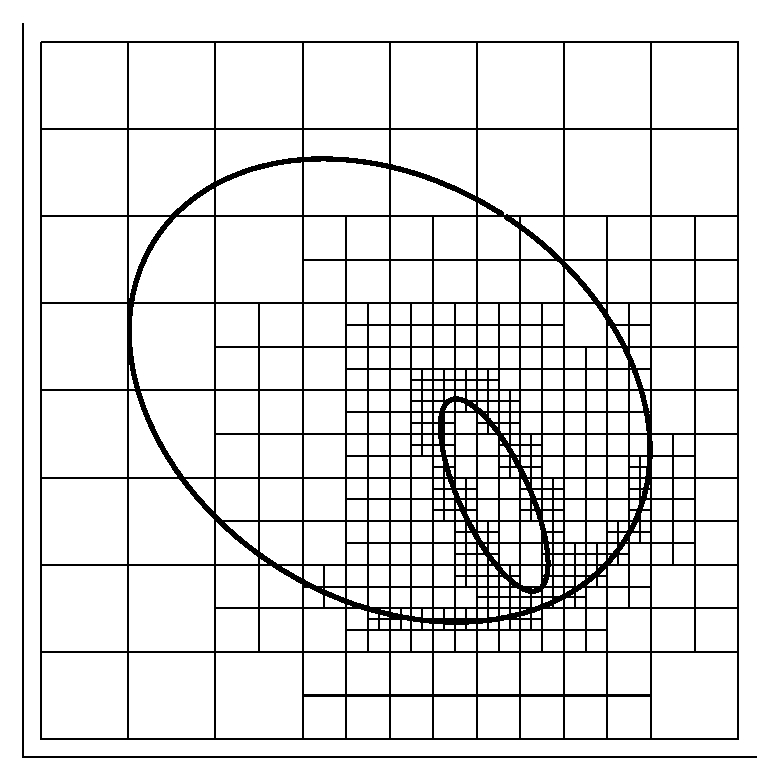
\includegraphics[height=2in]{figure2.eps} 
\end{array}$
  \caption{\em The domain for examples 1 and 4, including the quadtree structure for example 4. }
  \label{figure2}
\end{figure}
\noindent{\sc Example 1.}
The performance of the integral equation solver for\eqr{dirichlet:inteqn}  is carefully analyzed in \cite{KROP_QUAIFE_1}. In this example, we demonstrate some of the key features.
Here, we solve $u-\alpha^2 \Delta u = 0$, with $\alpha^2 = 0.1$ in an elliptical region containing an off-centre elliptical hole (see \figr{figure2}). The boundaries of the ellipses are described by $\y={\bf c} + (a\cos\phi\cos\alpha-b\sin\phi\sin\alpha,a\sin\phi\cos\alpha+b\cos\phi\sin\alpha)$. On $\Gamma_0$, ${\bf c} = {\bf 0}$, $a = 0.3$, $b = 0.4$, $\phi = 1$, and on $\Gamma_1$, ${\bf c} = (0.15,0.15)$, $a = 0.15$, $b = 0.05$, $\phi = 2$. We generate the boundary conditions from an exact solution,
\[
   u(\x) = K_0 \left( \frac{|\x - \x_1 |}{\alpha} \right), 
\]
 where $\x_1$ is a point inside $\Omega_1$. 
The performance on this example is shown in \tabr{table1}. Note that the number of GMRES iterations remains constant and the CPU time depends linearly on $N_\Gamma$.

\begin{table}[h]
  \centering
  \begin{tabular*}{\textwidth}{@{\extracolsep{\fill}}clcccc}
    \hline
    Max level & $h$ & $\mbox{Error}_1$ & $\mbox{Error}_2$ & $\mbox{Error}_3$ & $\mbox{CPU}_{\mbox{vol}}$ 
    \vspace{0.05in} \\
    \hline
    2 & 1/4 & $1.74 \times 10^{-4}$ & $5.80 \times 10^{-3}$ & $1.03 \times 10^{-4}$   & 0.11 \\
    3 & 1/8 & $3.51 \times 10^{-5}$ & $8.77 \times 10^{-5}$ & $8.26 \times 10^{-6}$   & 0.17 \\
    4 & 1/16 & $5.75 \times 10^{-6}$ & $3.08 \times 10^{-6}$ & $2.43 \times 10^{-6}$ &  0.27 \\
    5 & 1/32 & $1.89 \times 10^{-7}$ & $1.91 \times 10^{-7}$ & $7.62 \times 10^{-8}$ &  0.50 \\
    6 & 1/64 & $1.08 \times 10^{-7}$ & $5.34 \times 10^{-8}$ & $4.17 \times 10^{-9}$ &  1.35 \\
    7 & 1/128 & $1.55 \times 10^{-8}$ & $2.35 \times 10^{-9}$ & $8.20 \times 10^{-9}$ &  4.49 \\
\hline
  \end{tabular*}
 \caption{Performance of the volume potential solver on example 2. $\mbox{CPU}_{\mbox{vol}}$ is the time taken for the evaluation of the volume potential, measured in seconds.  $\mbox{Error}_1$ is the absolute error at $r=0.101$, $\mbox{Error}_2$ at $r=0.25$ and $\mbox{Error}_3$ at 0.399. A linear fit determines the decay rate of the error, $\mbox{Error}_k = O(h^p)$, where $p = 2.8$ for $k=1$, $p = 4.1$ for $k=2$ and $p=3.0$ for $k=3$. 
\label{table2} }
\end{table}

\begin{figure}[htps]
     \centering
$\begin{array}{cc}
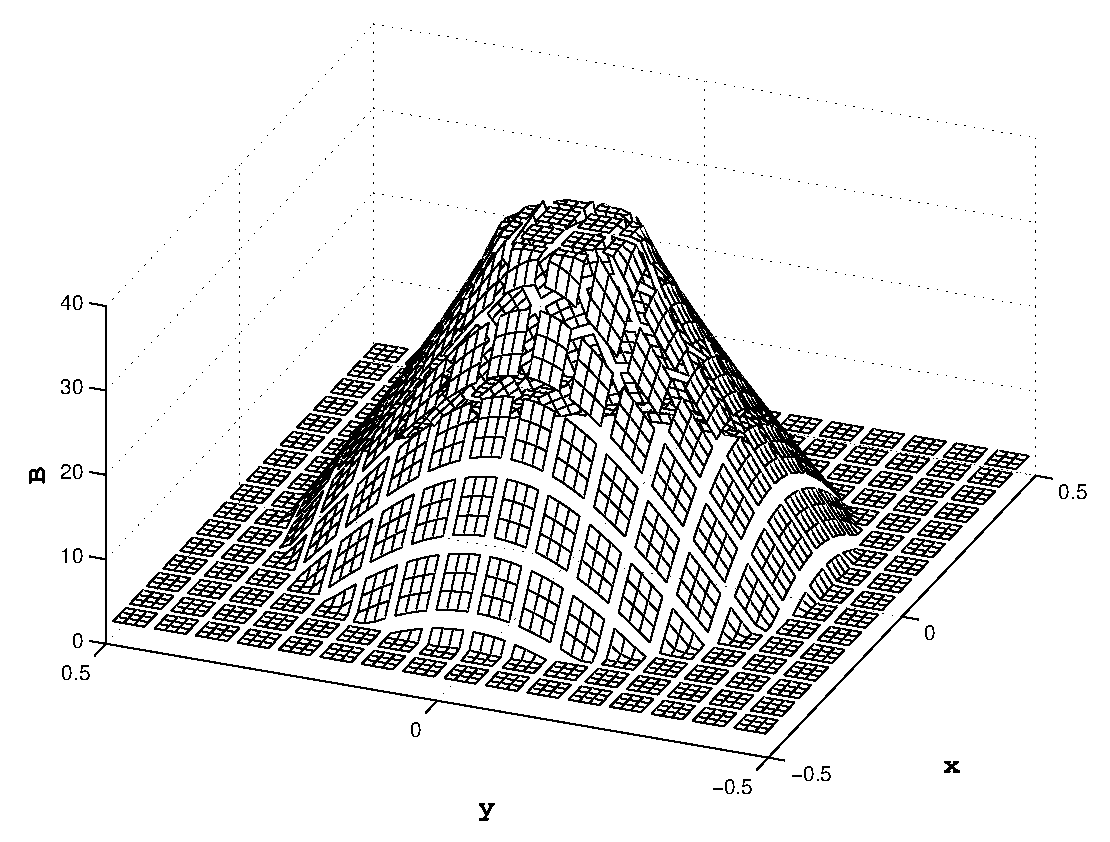
\includegraphics[height=2in]{figure3_a.eps} &
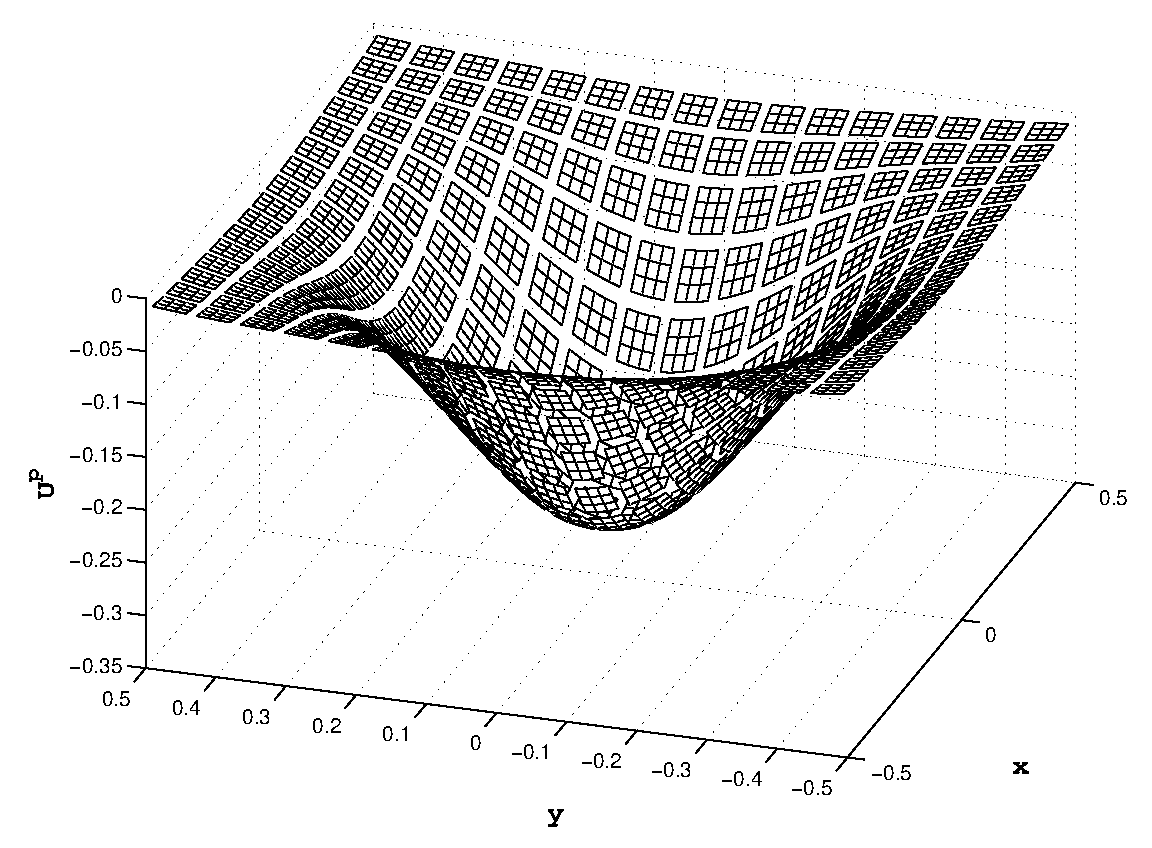
\includegraphics[height=2in]{figure3_b.eps}
\end{array}$
  \caption{\em The left plot shows $\tilde{B}$ for example 2 and the right is the corresponding volume potential. Here, the domain has been discretized with 4 levels of refinement. }
  \label{figure3}
\end{figure}
\noindent{\sc Example 2.} 
In this example, we test the spatial convergence for the volume potential solver (more details on its performance appear in \cite{modified:helmholtz}). We calculate solutions to $u - \alpha^2 \Delta u = B(\x)$, on the domain $\Omega$ bounded between $\Gamma_0$,  a circle of radius 0.4, and $\Gamma_1$, a circle of radius 0.1.
Here, we construct $B(r)$, $r = |\x|$,  and the boundary conditions to be chosen according to the exact solution
\[
u(r) = (r-0.4)^4 + r-0.4 \, . 
\]
We define a continuous extension of $B(r)$ defined throughout $D$ by
\[
\tilde{B}(r) = \left\{ \begin{array}{rl}
                                      B(r),      & \qquad \x \in \Omega, \\
                                      B(0.4),  & \qquad \x \in \Omega_0 \\
                                      B(0.1),  & \qquad \x \in \Omega_1.
                             \end{array}
                    \right. 
\]
A picture of this function throughout $D$ is shown in left-hand plot of \figr{figure3}. 
Each contour is discretized with 16384 points, which is large enough to ensure the error from the evaluation of the double layer potential is negligible. We discretize the domain $D$ with a uniform grid at varying levels of refinement and we calculate the maximum error at three different values of $r$, including 2 values that are 0.001 units away from the inner and outer boundaries.  The results are shown in \tabr{table2} and a picture of the volume potential is shown in right-hand plot of \figr{figure3}. As expected, we achieve 4th order convergence of the solution at the point that is well away from the physical boundaries. Close to $\Gamma_0$ and $\Gamma_1$, where $\tilde{B}$ has a discontinuity in its first derivative, the order of convergence drops closer to 3.  This is to be expected, and in order to achieve 4th order convergence throughout the domain, we would have to extend $B$ throughout $D$ to be at least ${\cal C}^1$ everywhere.

\begin{table}[htbp]
  \begin{center}
\begin{tabular*}{\textwidth}{@{\extracolsep{\fill}}ccc}
    \hline
  $ \Delta t$ & $\mbox{Error}_1$ & $\mbox{Error}_2$ \\  \hline
    $2.0 \times 10^{-3}$ & $1.37 \times 10^{-2}$ & $1.65 \times 10^{-3}$ \\
    $1.0 \times 10^{-3}$ &  $7.10 \times 10^{-3}$ & $4.74 \times 10^{-4}$ \\
    $5.0 \times 10^{-4}$ & $3.61 \times 10^{-3}$ & $1.24 \times 10^{-4}$ \\
    $2.5 \times 10^{-4}$ & $1.85 \times 10^{-3}$ & $3.23 \times 10^{-5}$ \\
    \hline
  \end{tabular*}
  \end{center}
\caption{The $\mathcal{L}_\infty$ error at $t=0.01$ using IMEX Euler ($\mbox{Error}_1$) and SBDF ($\mbox{Error}_2$) for example 2. (The error is measured at grid points inside the domain that are sufficiently far away from either boundary.) In this simulation, $N_\Gamma = 2048$, and volume grid is obtained by refining the unit square uniformly up to level 7 (i.e. the childless nodes are of size $1/128 \times 1/128$. This spatial resolution insures that the spatial error is negligible and the above errors are from the temporal discretization. 
\label{table3}  }
\end{table}
\noindent{\sc Example 3.} 
In this example, we solve the forced heat equation on a domain for which an analytical solution is known. 
The domain $\Omega$ is bounded between $\Gamma_0$,  a circle of radius 0.4, and $\Gamma_1$, a circle of radius 0.1. Both $\Gamma_0$ and $\Gamma_1$ are centered at the origin.
The forcing term is
\[
F(\x) = 400 \cos(20|\x|) + 20 \frac{\sin(20|\x|)}{|\x|}
\]
The following is the exact solution to the heat equation:
\begin{align*}
  u(x,t)=e^{-\lambda^{2}t}\left[Y_{0}(0.1\lambda)J_{0}(\lambda|\x|)-
  J_{0}(0.1\lambda)Y_{0}(\lambda|\x|)\right]+\cos (20 |\x|), 
\end{align*}
where $J_0$ is the zeroth-order Bessel function of the first kind, and $Y_0$ is the zeroth-order Bessel function of the second kind. 
We have chosen $\lambda$ so that the time-dependent term vanishes on both boundaries $\lambda \approx 10.244$. 
The boundary conditions, then, are 
\[
   f(\x) = \left\{ \begin{array}{rl}
                            \cos(8), & \qquad \x \in \Gamma_0, \\
                            \cos(2), & \qquad \x \in \Gamma_1.
                         \end{array} \right.
\]
We calculate solutions to the heat equation using the IMEX Euler and SBDF methods, up to $t = 0.01$. The spatial resolution is high enough that the spatial error is negligible in comparison to the temporal error. The results are summarized in \tabr{table3}. As shown in this table, we achieve first and second-order convergence for the Euler and SBDF methods, respectively. 

\begin{table}[h]
  \centering
\begin{tabular*}{\textwidth}{@{\extracolsep{\fill}}lrrrrr}
    \hline
    $\tau$ & $N_D$ & $\mbox{CPU}_{\mbox{tree}}$ & $\mbox{CPU}_{\mbox{lay}}$ & $\mbox{CPU}_{\mbox{int}}$ 
    & $\mbox{CPU}_{\mbox{total}}$ \vspace{0.05in} \\ 
    \hline
    $10^{-4}$   & 6064   & 19.27 & 38.80   & 329.93 & 410.51   \\
    $10^{-6}$   & 13696 & 56.22 & 57.10   & 330.10 & 491.32   \\
    $10^{-8}$   & 33712 & 140.38 & 86.14   & 329.55 & 657.04 \\
    $10^{-10}$ & 67840 & 203.54 & 125.96 & 329.80 & 834.83 \\
    $10^{-12}$ & 94912 & 238.79 & 148.29 & 328.36 & 945.66 \\

    \hline
  \end{tabular*}
\caption{A break down in the CPU time (in seconds) for the 100 time steps taken in the solution to Example 4. $N_D = 16 P$, where $P$ is the total number of childless boxes as determined by the interpolation error tolerance $\tau$. The total number of points on the boundary is $N_{\Gamma} = 1024$. $\mbox{CPU}_{\mbox{tree}}$ is the time taken for the generation of the initial quadtree, $\mbox{CPU}_{\mbox{lay}}$ is the total time taken for all evaluations of the layer potential at the $N_D$ grid points, $\mbox{CPU}_{\mbox{int}}$ is the total time taken for the solution to all integral equations (12 GMRES iterations were required at each time step to solve the integral equation).
\label{table4} }
\end{table}
\noindent{\sc Example 4.} In this example, we solve the homogeneous heat equation in an elliptical region containing an off-center elliptical hole (the same geometry as in example 1).  The initial condition is homogeneous, and the boundary conditions are
\[
   f(\x) = \left\{ \begin{array}{rl}
                            0, & \qquad \x \in \Gamma_0, \\
                            1, & \qquad \x \in \Gamma_1.
                         \end{array} \right.
\]
The quadtree structure for the solution at the first time step is shown in \figr{figure2} and a break down of the computational cost is shown in \tabr{table4}. The bulk of the computation costs come from the generation of the quadtree, the evaluation of the layer potential at the volume grid points and the solution to the integral equation. The total computational cost is $O(N_D)$, as expected. Plots of the solution at three different times are shown in \figr{figure4}. At the final time, the solution is near steady state. 

\begin{figure}[htps]
     \centering
$\begin{array}{cc}
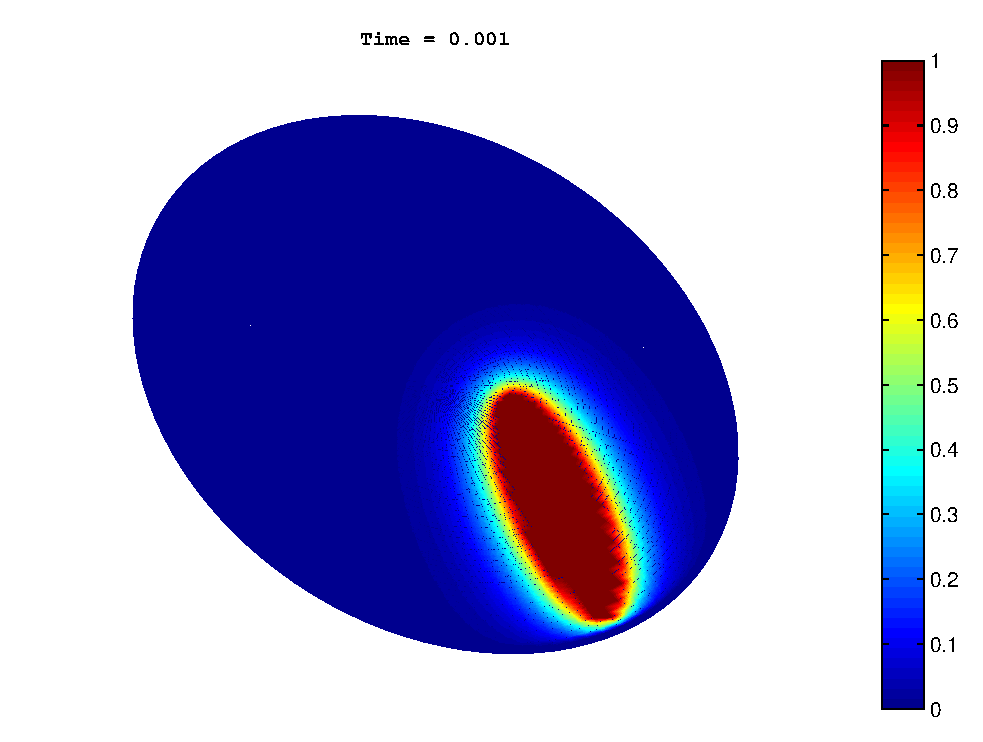
\includegraphics[height=1.75in]{figure4_a.eps} &
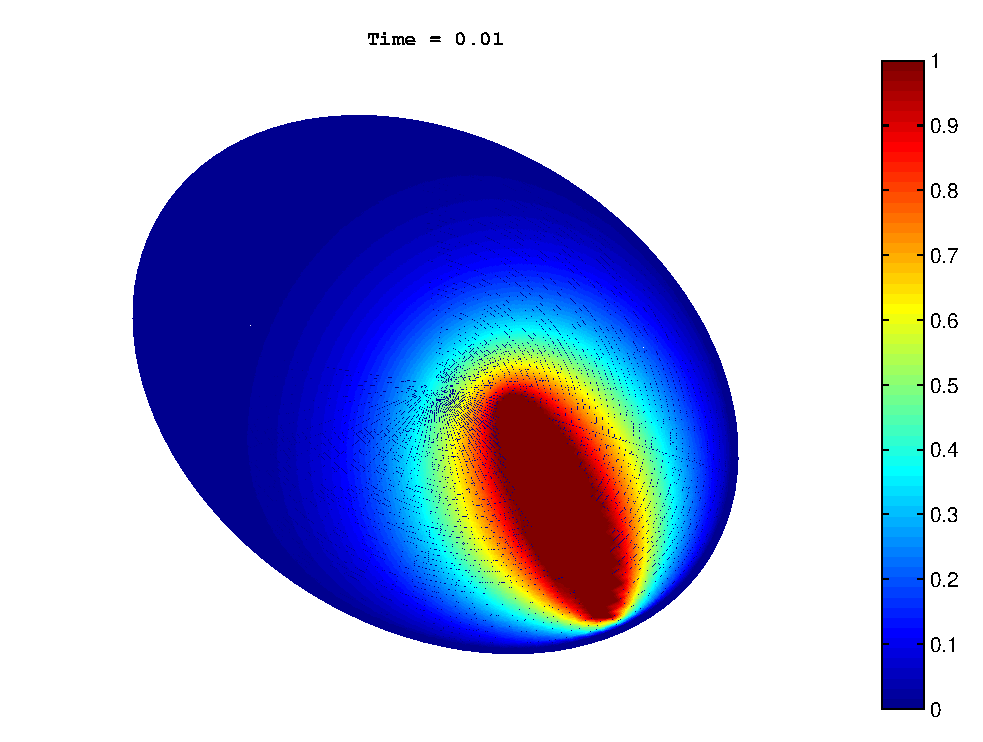
\includegraphics[height=1.75in]{figure4_b.eps} \\
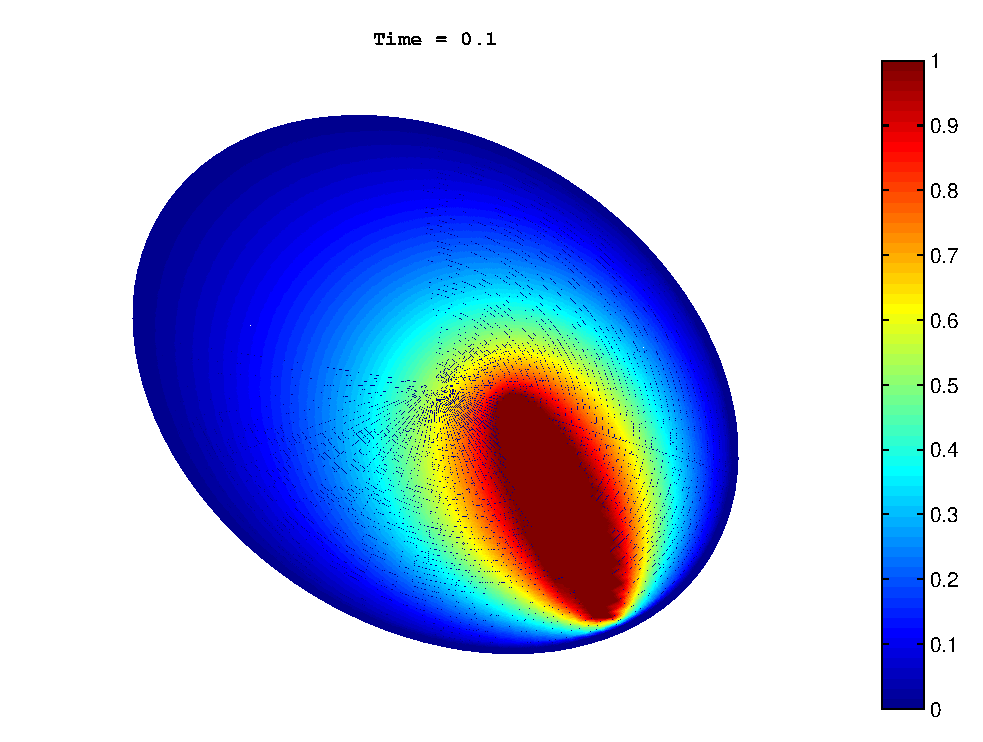
\includegraphics[height=1.75in]{figure4_c.eps} 
\end{array}$
  \caption{\em The solution to example 4 at three different times. }
  \label{figure4}
\end{figure}

\begin{figure}[htps]
     \centering
$\begin{array}{cc}
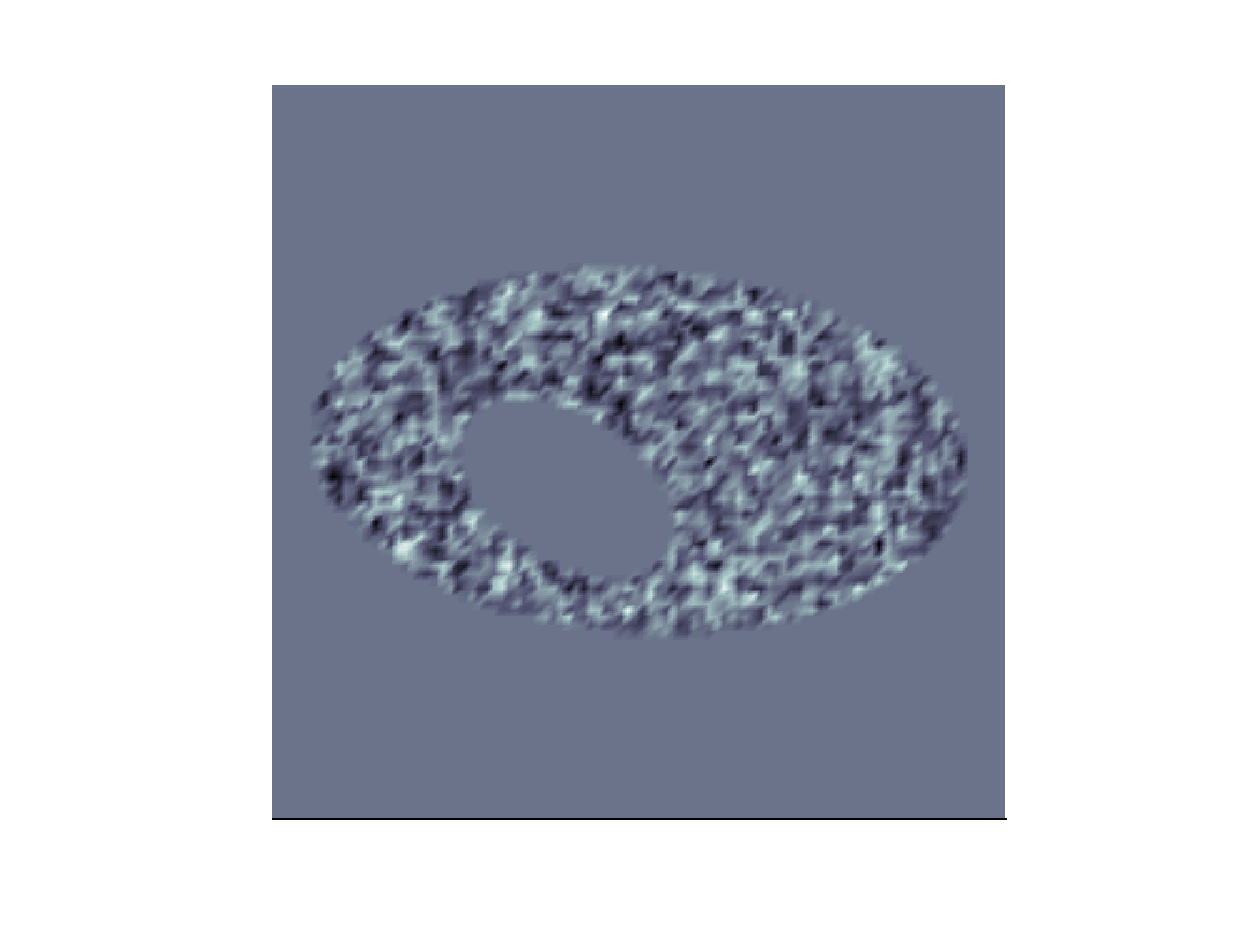
\includegraphics[height=1.75in]{figure5_a.eps} &
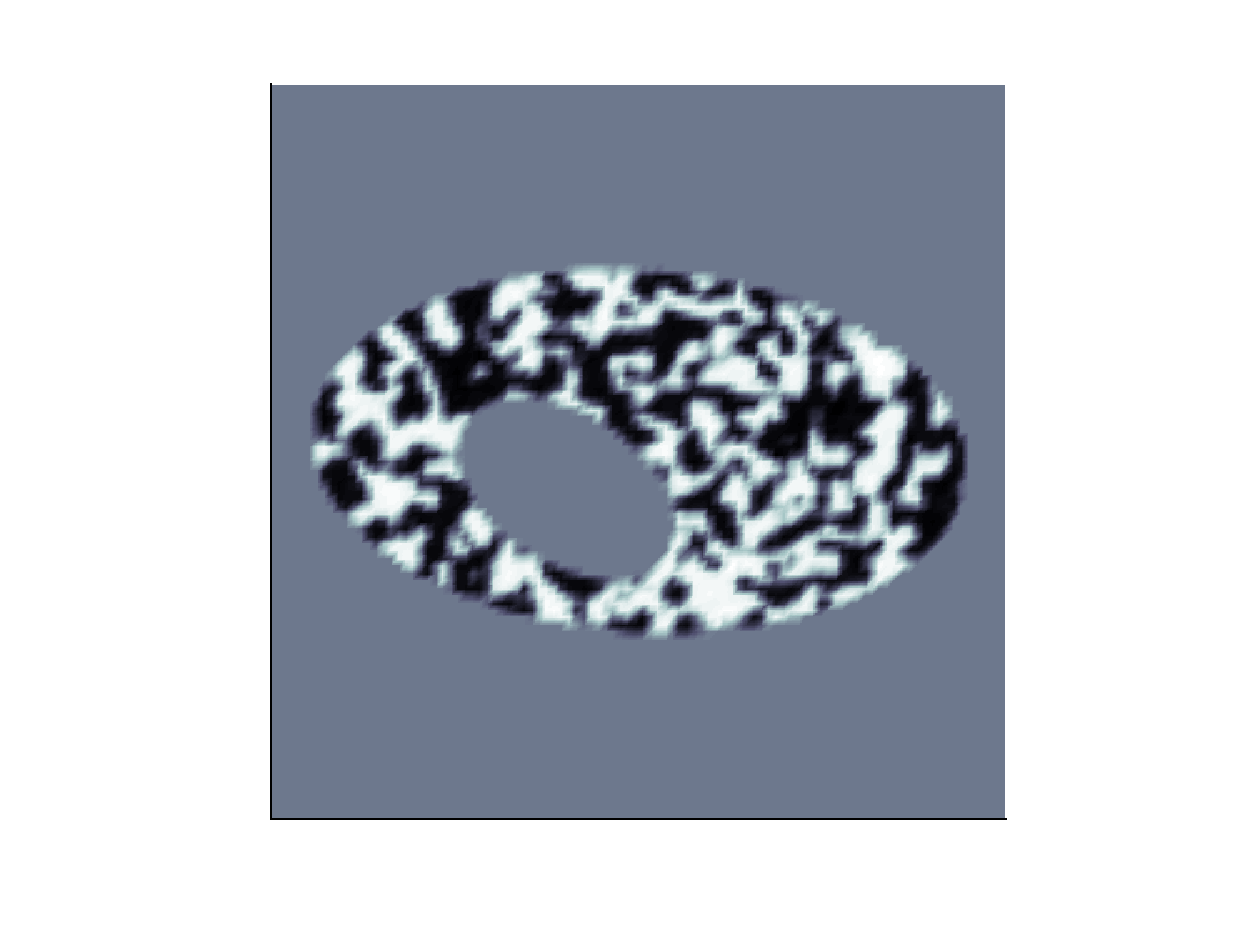
\includegraphics[height=1.75in]{figure5_b.eps} \\
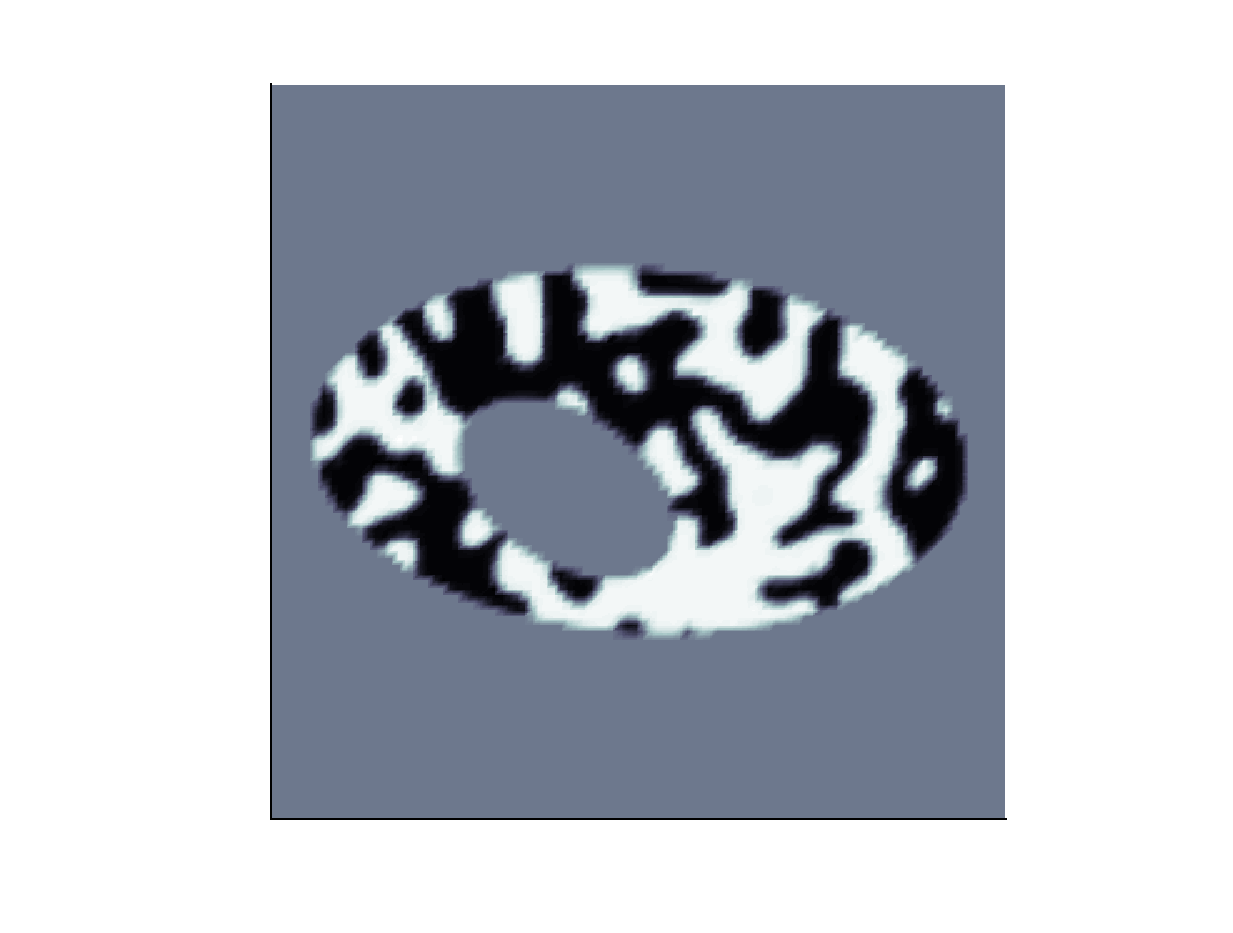
\includegraphics[height=1.75in]{figure5_c.eps} &
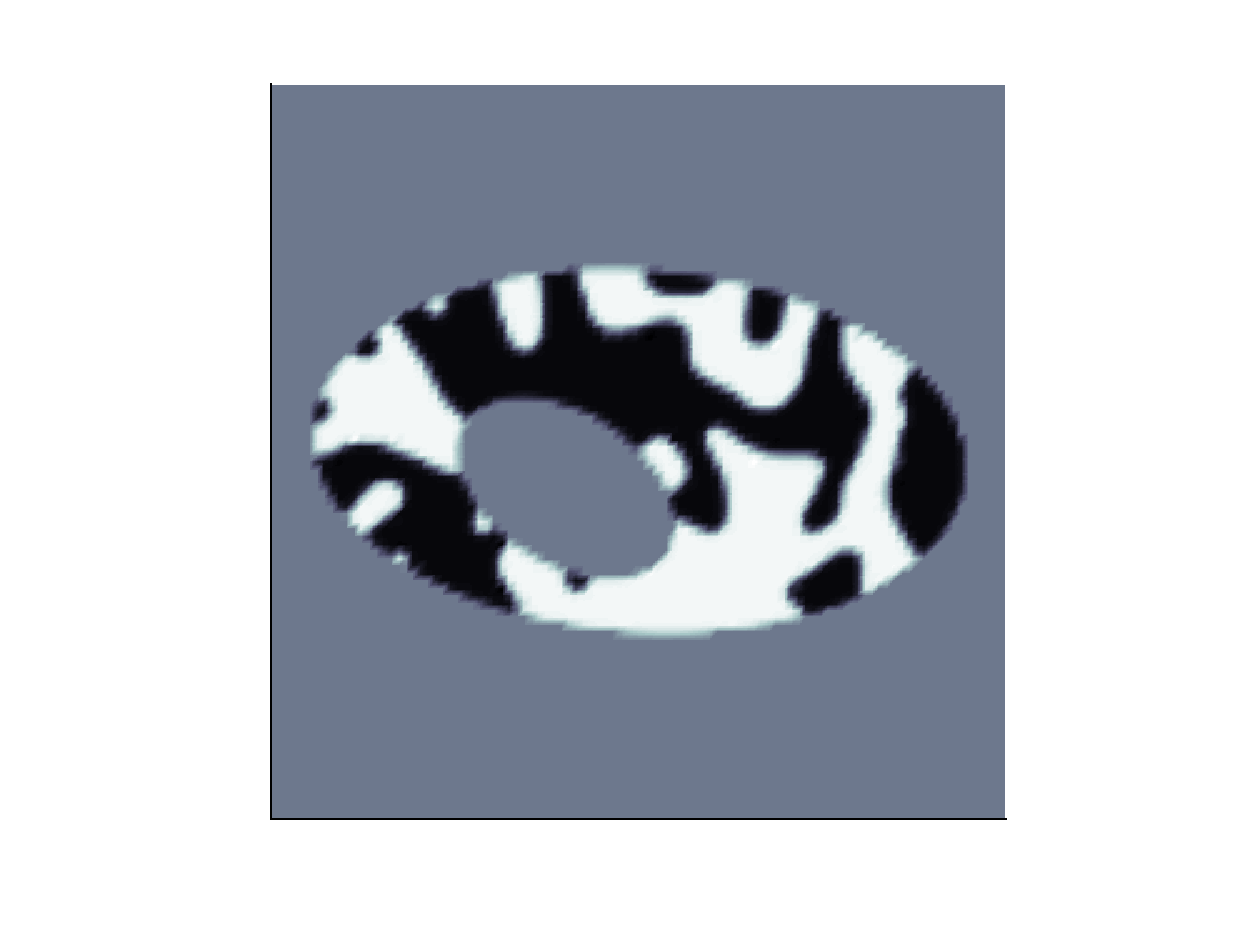
\includegraphics[height=1.75in]{figure5_d.eps} 
\end{array}$
  \caption{\em The solution to Example 5. Here, $\Delta t = 1$ and IMEX Euler's method is used. The unit square is uniformly refined to level 6 (i.e. the finest boxes are of size $1/64 \times 1/64$. The upper left plot is at $t=0$, and proceeding clockwise, the remaining plots are at $t=13$, $t=43$, and $t=100$, respectively. }
  \label{figure5}
\end{figure}

\noindent{\sc Example 5.}
In this example, we demonstrate that our methods can be applied to much more complex equations. 
Here, we solve the Allen-Cahn equation 
\begin{align*}
   u_t - \epsilon \Delta u & =  u(1-u^2), &   \x \in \Omega, \; t>0, \\
   u(\x,t) & =   0, & \x \in \Gamma_0,  \\
   u(\x,t) & =  0,  &  \x \in \Gamma_1,
\end{align*}
where $\epsilon = 10^{-5}$. 
We initialize the solution with random values uniformly distributed on $[-1/2, 1/2]$.  
The nonlinear forcing term is evaluated explicitly in the time stepping and is incorporated into the right-hand side of equation\eqr{mod_helm_forced}. 
The general behaviour of solutions to the Allen-Cahn equation is well known: 
the stable stationary solutions are $u=1$ and $u=-1$ and the solution exhibits coarsening towards these values.
The presence of physical boundaries can create more complex patterns, as seen in \figr{figure5} and \figr{figure6}. 
In computing the solutions to processes involving coarsening or pattern formation behaviour, it would be desirable to adapt the quadtree on the fly, so as to ensure adequate resolution for changing solution features within the domain. This will be considered in the future.

\begin{figure}[htps]
     \centering
$\begin{array}{cc}
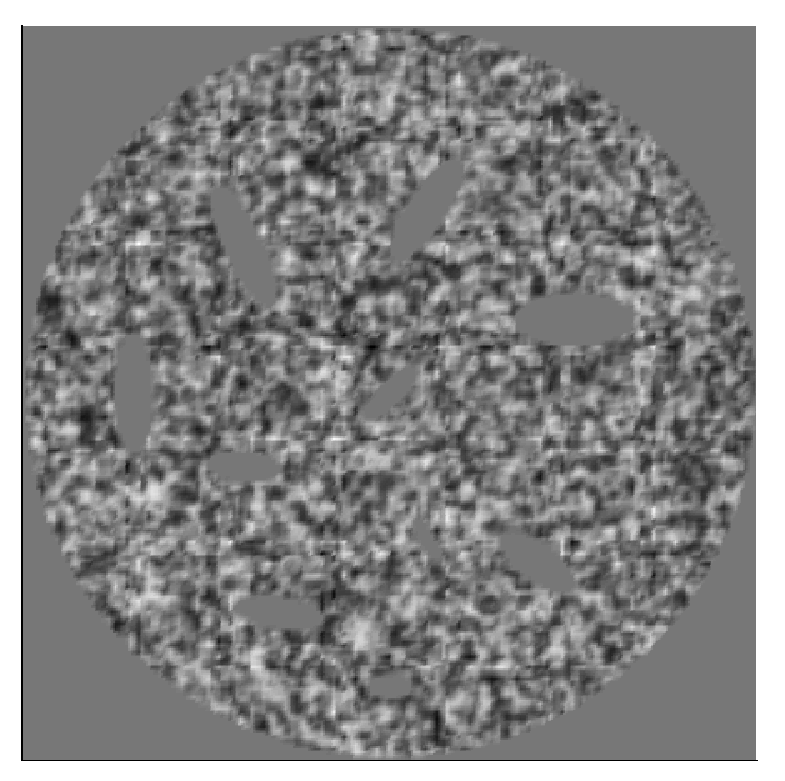
\includegraphics[height=1.75in]{figure6_a.eps} &
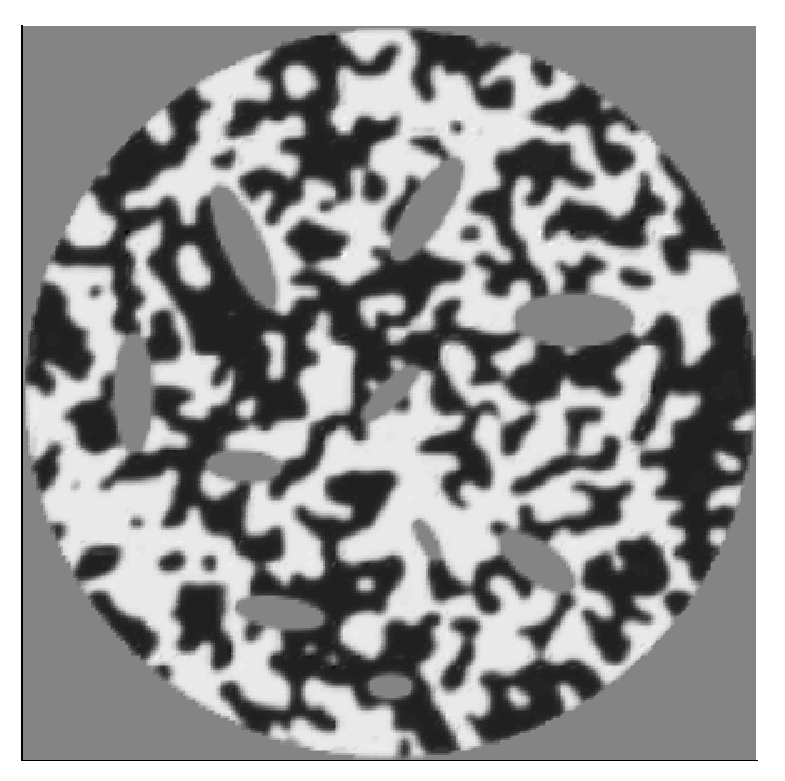
\includegraphics[height=1.75in]{figure6_b.eps} \\
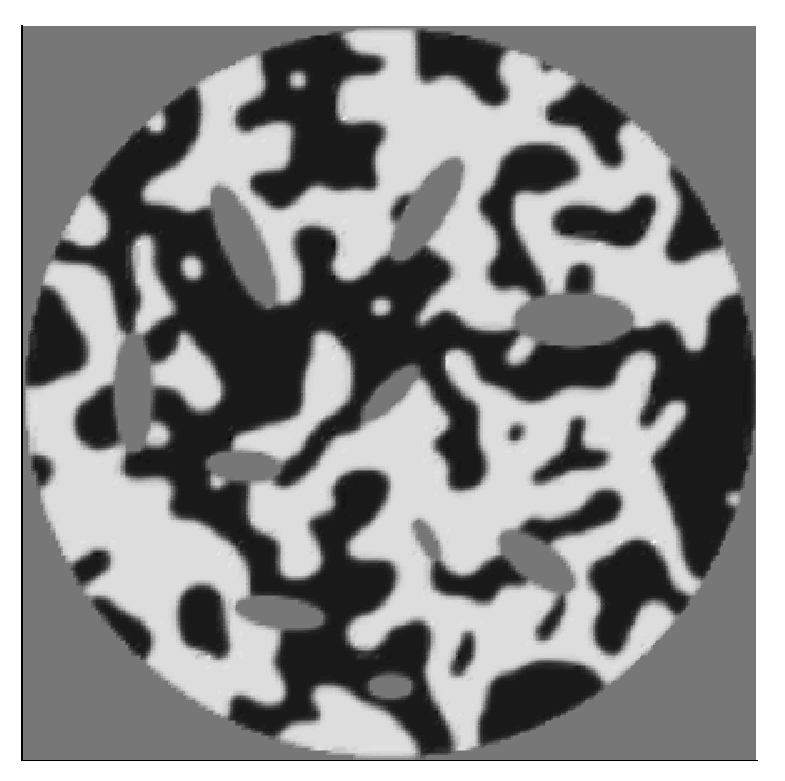
\includegraphics[height=1.75in]{figure6_c.eps} &
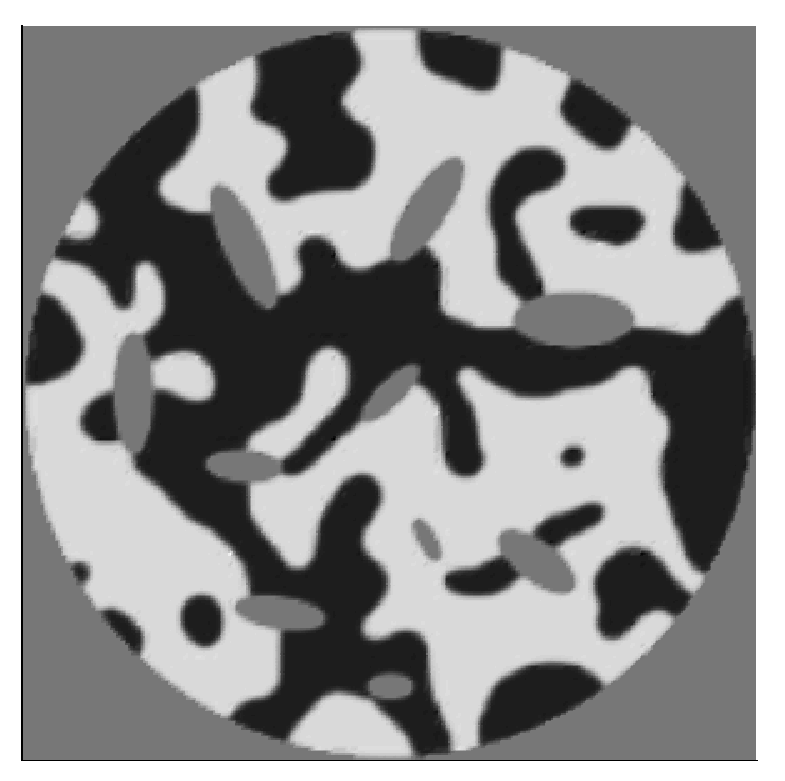
\includegraphics[height=1.75in]{figure6_d.eps} 
\end{array}$
  \caption{\em The solution to example 5 in a domain with 10 interior component curves.  Here, $N_\Gamma = 2816$, $N_D = 65,536$, $\Delta t = 1$, and 100 time steps are taken. Total CPU time of approximately 19.5 minutes.  The upper left plot is at $t=0$, and proceeding clockwise, the remaining plots are at $t=13$, $t=43$, and $t=100$, respectively.}
  \label{figure6}
\end{figure}

%%%%%%%%%%%%%%%%%%%%%%%%%%
%\begin{center}
\section{Conclusions}
We have presented an investigation on coupling available fast algorithms for the modified Helmholtz equation for the purposes of solving the isotropic, nonlinear heat equation.  
We base our approach on Rothe's method: we discretize in time first and then use integral equation methods to solve a sequence of elliptic boundary value problems.  
We have demonstrated the methods on a number of examples and have shown that this approach has potential to efficiently and accurately solve the heat equation in complicated geometry. One important aim of this paper was to identify and elucidate the remaining issues that need to be resolved in order to develop this approach into a fully general solver.
These issues are listed below:
\begin{itemize}
\item The extension of $B(\x,u,t)$ throughout the computational domain $D$ for general boundary conditions $u = f(\x)$ and forcing term $F(\x,u,t)$ remains an open problem. Based on our results, it may be sufficient to do a ${\cal C}^0$ extension only, although a ${\cal C}^1$ is desirable. This may be achievable by local interpolation, or by solving a suitable integral equation inside each $\Omega_k$ and outside $\Omega_0$.
\item In order to appropriately resolve solution features that appear/disappear within the domain, it may be necessary to dynamically generate the quadtree throughout the simulation. However, the cost of generating of the quadtree is nontrivial and this would have to be done carefully in order to maintain efficiency. 
\item The integral operator of the double layer potential becomes singular at grid points in $D$ close to $\Gamma$. Our approach here was to simply over-resolve the boundary grid. A more desirable approach would be to incorporate special quadratures, possibly using the ones discussed in \cite{beale,strain}. 
\end{itemize}

Once these issues have been addressed and a fully general solver has been developed, we plan on using this solver to study complex reaction-diffusion systems. We also plan to develop similar integral equation methods for the incompressible Navier-Stokes equations.
Future work will also include examining alternative temporal discretization methods. 
For instance, one promising avenue would be to combine the fast solver for the modified Helmholtz equation with a spectral-deferred correction, time-integration scheme \cite{dutt,jia_huang} in order to achieve both a high degree of accuracy and unconditional stability. 
Future work will also include moving into three dimensions.  
This will require careful consideration of an appropriate quadrature and a suitable representation for surfaces. However, a a fast multipole method already exists for the three-dimensional screened Coulomb potential in three dimensions \cite{screened_coulomb}.


\noindent
{\bf Acknowledgements:}
 The authors wish to thank Rustum Choksi and Yves Van Gennip for their help with example 5, and Jingfang Huang for his considerable help with his volume potential solver. 
%\end{center}
\bibliographystyle{plain}
\begin{thebibliography}{10}

\bibitem{ABRAM}
M.~Abramowitz and I.A. Stegun.
\newblock {\em Handbook of Mathematical Functions}.
\newblock Dover, New York, NY, 1964.

\bibitem{alpert:quad:rules}
Bradley Alpert.
\newblock Hybrid Gauss-trapezoidal quadrature rules.
\newblock {\em SIAM J. Sci. Comp.}, 20:1551--1584, 1999.

\bibitem{Ruuth}
U.M. Ascher, S.J. Ruuth, and B.M. Wetton.
\newblock Implicit-explicit methods for time-dependent partial differential
  equations.
\newblock {\em SIAM J. Numer. Anal.}, 32:797--823, 1995.

\bibitem{beale}
J.~Thomas Beale and Ming-Chih Lai.
\newblock A method for computing nearly singular integrals.
\newblock {\em SIAM J. Numer. Anal.}, 38(6):1902--1925, 2001.

\bibitem{GB_LY_DZ}
George Biros, Lexing Ying, and Denis Zorin.
\newblock An embedded boundary integral solver for the unsteady incompressible
  {N}avier-{S}tokes equations.
\newblock preprint, (2002).

\bibitem{BIROS}
George Biros, Lexing Ying, and Denis Zorin.
\newblock A fast solver for the Stokes equations with distributed forces in
  complex geometries.
\newblock {\em J. Comp. Phys.}, pages 317--348, 2003.

\bibitem{CGR}
J.~Carrier, L.~Greengard, and V.~Rokhlin.
\newblock A fast adaptive multipole algorithm for particle simulations.
\newblock {\em SIAM J. Sci. Statist. Comput.}, 9:669--686, 1988.

\bibitem{chapko}
Roman Chapko.
\newblock On the combination of {R}othe's method and boundary integral
  equations for the nonstationary stokes equations.
\newblock {\em J. Integral Equations and Appl.}, 13(2), 2001.

\bibitem{chapko_kress}
Roman Chapko and Rainer Kress.
\newblock {R}othe's method for the heat equation and boundary integral
  equations.
\newblock {\em J. Integral Equations and Appl.}, 9(1):47--69, 1997.

\bibitem{modified:helmholtz}
H.~Cheng, J.~Huang, and T.~Leiterman.
\newblock An adaptive fast solver for the modified Helmholtz equation in two
  dimensions.
\newblock {\em J. Comp. Phys.}, 211:616--637, 2006.

\bibitem{dutt}
S.~Dutt, L.~Greengard, and V.~Rokhlin.
\newblock Spectral deferred correction methods for ordinary differential equations.
\newblock {\em BIT}, 40(2):241--266, 2000.

\bibitem{greengard:ethridge}
F.~Ethridge and L.~Greengard.
\newblock A new fast-multipole accelerated Poisson solver in two dimensions.
\newblock {\em SIAM J. Sci. Comp.}, 23(3):741--760, 2001.

\bibitem{mult:conn}
A.~Greenbaum, L.~Greengard, and G.B. McFadden.
\newblock {L}aplace's equation and the Dirichlet-Neumann map in multiply
  connected domains.
\newblock {\em J. Comp. Phys.}, 105:267--278, 1993.

\bibitem{screened_coulomb}
L.~Greengard and J.~Huang.
\newblock A new version of the fast multipole method for screened Coulomb
  interactions in three dimensions.
\newblock {\em J. Comp. Phys.}, 180:642--658, 2002.

\bibitem{int:equation:nse}
L.~Greengard and M.C. Kropinski.
\newblock An integral equation approach to the incompressible {N}avier-{S}tokes
  equations in two-dimensions.
\newblock {\em SIAM J. Sci. Comp.}, 20:318--336, 1998.

\bibitem{stokes:flow}
L.~Greengard, M.C. Kropinski, and A.~Mayo.
\newblock Integral equation methods for stokes flow and isotropic elasticity in
  the plane.
\newblock {\em J. Comp. Phys.}, 125(2):403--414, 1996.

\bibitem{GR}
L.~Greengard and V.~Rokhlin.
\newblock A fast algorithm for particle simulations.
\newblock {\em J. Comp. Phys.}, 73:325--348, 1987.

\bibitem{new_FMM}
L.~Greengard and V.~Rokhlin.
\newblock A new version of the fast multipole method for the {L}aplace equation
  in three dimensions.
\newblock {\em Acta Numer.}, 6:229--269, 1997.

\bibitem{jia_huang}
J.~Jia and J.~Huang.
\newblock Krylov deferred correction accelerated method of lines transpose for parabolic systems".
\newblock {\em J. Comp. Phys.}, 227(3):1739--1753, 2008.

\bibitem{KROP_QUAIFE_1}
M.C. Kropinski and B.~Quaife.
\newblock Integral equation methods for the modified Helmholtz equation.
\newblock {\it J. Comp. Phys.}, 230:425--434, 2011.

\bibitem{heat_solver_1}
Jing-Rebecca Li and Leslie Greengard.
\newblock On the numerical solution of the heat equation {I}: Fast solvers in
  free space.
\newblock {\em J. Comp. Phys.}, 226:1891--1901, 2007.

\bibitem{heat_solver_2}
Jing-Rebecca Li and Leslie Greengard.
\newblock High order accurate methods for the evaluation of layer heat
  potentials.
\newblock {\em SIAM J. Sci. Comput.}, 31(5):3847--3860, 2009.

\bibitem{mayo}
Anita Mayo.
\newblock The fast solution of Poisson's and the Biharmonic equations on
  irregular regions.
\newblock {\em SIAM J. Numer. Anal.}, 21(2):285--289, 1984.

\bibitem{MAYO_2}
Anita Mayo.
\newblock Rapid, fourth order accurate solution of the steady Navier Stokes
  equations on general regions.
\newblock {\em Dyn. Contin. Discrete Impuls. Syst. Ser. B Appl. Algorithms},
  12:59--72, 2005.

\bibitem{mayo_greenbaum}
Anita Mayo and Anne Greenbaum.
\newblock Fourth order accurate evaluation of integrals in potential theory on
  exterior 3D regions.
\newblock {\em J. Comp. Phys.}, 220:900--914, 2007.

\bibitem{nishimura}
N.~Nishimura.
\newblock Fast multipole accelerated boundary integral equation methods.
\newblock {\em Appl. Mech. Rev.}, 55(4):299--324, July 2002.

\bibitem{SAAD}
Y.~Saad and M.H. Schultz.
\newblock {GMRES}: a generalized minimum residual algorithm for solving
  nonsymmetric linear systems.
\newblock {\em SIAM J. Sci. Stat. Comput.}, 7:856--869, 1986.

\bibitem{strain}
J.~Strain.
\newblock Locally-corrected multidimensional quadrature rules for singular
  functions.
\newblock {\em SIAM J. Sci. Comp.}, 6(4):992--1017, 1995.

\bibitem{tausch}
Johannes Tausch.
\newblock A fast method for solving the heat equation by layer potentials.
\newblock {\em J. Comp. Phys.}, 224:956--969, 2007.

\bibitem{SKVandGB}
Shravan~K. Verrapaneni and George Biros.
\newblock A high-order solver for the heat equation in 1D domains with moving
  boundaries.
\newblock {\em SIAM J. Sci. Stat. Comp.}, 29(6):2581--2606, 2007.

\bibitem{SKVandGB2}
Shravan~K. Verrapaneni and George Biros.
\newblock The Chebyshev fast Gauss and nonuniform fast Fourier transforms and
  their application to the evaluation of distributed heat potentials.
\newblock {\em J. Comp. Phys.}, 227:7768--7790, 2008.

\end{thebibliography}
%\bibliography{/Users/MC/Documents/Papers/mcak_bib}
\end{document}
